% \section{Large-scale Empirical Study and Discoveries}
\chapter{大规模实证研究与发现}
\label{chp:discoveries}

With the large-scale dataset ready, we can further conduct a comprehensive empirical study to acquire the nature of fake apps as well as understanding their ecosystem.
在大规模数据库准备好之后,我们可以
To effectively measure different facades of fake apps, We define three perspectives, namely \emph{Fake Sample Characteristics}, \emph{Quantitative Study on Fake Samples}, and \emph{Developing Trend}.
Next, we'll describe each perspective in detail.

% \subsection{Fake Sample Characteristics}
\section{Fake Sample Characteristics}
To reveal the strategy the fake app authors are employing, or how they bypass app markets' security scheme, fake sample characteristics have to be understood.
As such, we conduct our measurement in terms of certificates and basic information like app names, package names and package sizes.

Certificate serves as the identifier for developers.
The nature of the certificate, namely, whether each fake app has a unique certificate, is likely to be essential to fake apps' evasive technique.
On the other hand, we believe repackaged apps, as a kind of \texttt{imposters}, are widespread in our dataset.
Measurement on basic information of fake apps, such as package names and package sizes, helps us determine how repackaged apps are distributed, since repackaging an app does not change any of its basic information (i.e. the app name, package name, version code, etc.) unless it's done intentionally.

To this end, we have some hypotheses as below:

\noindent{\bf Hypo 1.1:} Most of these fake samples have their corresponding unique certificates.
In other words, most fake certificates and fake samples have a one-to-one relation.

\noindent{\bf Hypo 1.2:} A large portion of fake samples have the same app names/package names/apk sizes as those in official samples.

To verify our hypotheses as well as to gain knowledge to fake sample individuals, we propose the following research questions in this subsection.

\noindent{\bf RQ 1.1}: What's the relationship between the number of fake samples and their certificates? That is, how many fake samples does one certificate usually link to?

\noindent{\bf RQ 1.2}: How do fake apps imitate official apps? That is, how similar are the names/package names/apk sizes of fake samples compared to those of official samples?

\begin{figure*}[htbp]
	\centering
    \subfloat[应用名\label{fig:appname}]{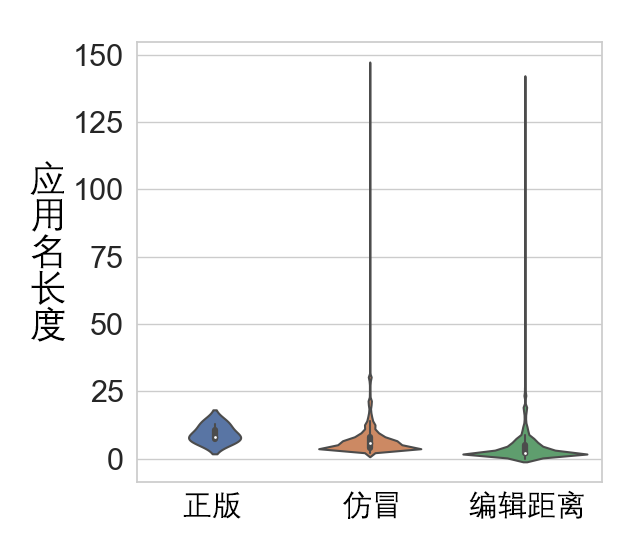
\includegraphics[width=0.33\textwidth]{./Figures/edwin-RQ1-2(a).png}}\hfill
    \subfloat[包名\label{fig:pkgname}]{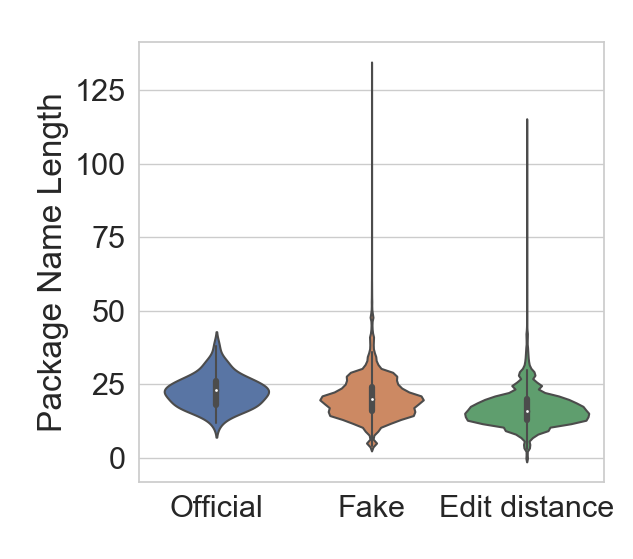
\includegraphics[width=0.33\textwidth]{./Figures/edwin-RQ1-2(b).png}}\hfill
    \subfloat[样本大小\label{fig:size}]{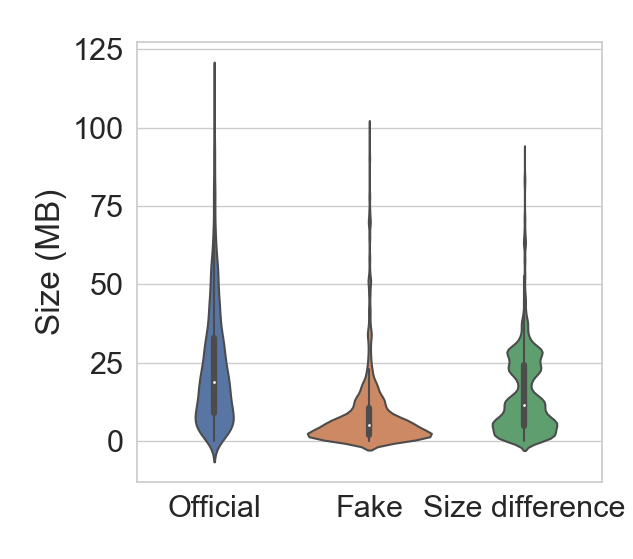
\includegraphics[width=0.33\textwidth]{./Figures/edwin-RQ1-2(c).png}}\hfill
	\caption{对App各项属性的统计结果}
	\label{fig:Statistic_fake_and_official}
	\vspace{-5mm}
\end{figure*}

\noindent{\bf Answer to RQ 1.1.}
76\% of these fake certificates are linked to merely one or two fake samples, and the number of fake examples a certificate links to is various from 1 to 1,374.
We count the number of certificates which link to different sample number in table~\ref{table:certificate_number_statistic}.

\begin{table}
  \renewcommand{\arraystretch}{1}
  \footnotesize
  \centering
  \caption{Statistics on fake samples and their certificates}
  \vspace{1mm}
  \begin{tabular}{l c c c c c c c}
  \toprule
  {\bf \# of samples} & {\bf 1-5} & {\bf 6-10} & {\bf 11-50} & {\bf 51-100} & {\bf More than 100} \\
  \midrule
  {\bf \# of certificates} & 8252 & 525 & 531 & 71 & 80 \\
  \bottomrule
  \end{tabular}
  \label{table:certificate_number_statistic}
\end{table}

This discovery partly matches our assumption that most of these fake samples have their corresponding unique certificates.
We consider this as a strategy to bypass app markets' security scheme, as even if one fake sample is exposed, other fake samples developed by the same developer will not be implicated directly.
Nevertheless, when reviewing certificates linked with multiple fake samples, we find some very surprising findings that we will expound in Section~\ref{sec:casestudy}.

\noindent{\bf Answer to RQ 1.2.}
According to our statistical result, only 243 out of 52,638 samples (less than 0.5\%) use official package names, all the rest fake samples (more than 99.5\%) use their own package names.
In the rest 52,395 samples, 14,089 different package names were found.
But does this mean fake samples are all using package names that are totally different from the official ones? Could they be using package names that are similar to their official correspondences?

To figure out the similarity, we utilize \textit{edit distance}~\cite{levenshtein1966binary}, a distance definition widely applied in natural language processing (NLP):
{Given two strings $a$ and $b$, the edit distance $d(a, b)$ is the minimum-weight series of edit operations that transform $a$ into $b$.
In our case, edit operations refer to either to append, to delete or to change a character.}
For instance, the edit distance between string ``fake" and ``official" is 7, while between ``jingdong" and ``jindeng", this value becomes 2.
For every fake package name from a fake sample, we compute its edit distance to the official package name of its original.

Fig.~\ref{fig:Statistic_fake_and_official} is consist of three violin plots,\footnote{\url{https://en.wikipedia.org/wiki/Violin_plot/}} representing our statistics on app names, package names and package sizes, respectively.
In each ``violin'', the white dot represents the median, the thick bar in the middle represents the interquartile range while the thin bar represents 95\% confidence interval.

Fig.~\ref{fig:appname} shows the statistic information on app names of official samples, fake samples, and the edit distance between them.
Both the white dot in ``Official'' violin and the one in ``Fake'' violin are at a similar level near the value ``6'', which means the average length of app names of both official samples and fake samples are close to each other.
The overall distribution of these two data groups have similar bodies, signals that they are also similar as well.
What's more, the median value of edit distance is low (``2'' on $y$-axes), meaning that half of the fake apps get their names by modifying less than 3 characters from the corresponding official apps' names.
This is a proof indicating that most fake apps are using a similar name to an official name.
At the same time, we notice that some fake apps have pretty long names (there is one with a name of 146-character-long length).
Many of those outliers are samples uploaded by fake authors, maybe for testing purpose to explore the vetting mechanism. The other purpose is to associate users' search keywords as far as possible.

Fig.~\ref{fig:pkgname} shows the result on package names.
Like the plots in Fig.~\ref{fig:appname}, the difference between the average length of package names of official apps and the average length of package names of fake apps is still tiny (they are of value ``23'' and ``20'', respectively).
Nonetheless, the median of edit distance between them is explicitly higher (``16'' on $y$-axes), which means it takes averagely 16 times modification to turn a fake package name to an official package name and vice versa.
Thus, we infer that fake apps tend to use self-defined package names.

Fig.~\ref{fig:size} reports package size information.
To better represent the trend, we eliminated some outliers: samples that are larger than 150MB (851 in 69,614 official samples (about 1\%) and 447 in 52,638 fake samples (less than 1\%), most of which are from 游戏 category).
The figure shows that the median number of fake samples' size is around 5MB, while half of the official apps have a size greater than 18MB, meaning that fake apps are more likely to be
(1) developed by their owners but not originated from repackaging official apps,
(2) malicious apps, for malicious apps are usually in small sizes.

In short, Fig.~\ref{fig:Statistic_fake_and_official} tells that fake apps
(1) prefer to use a similar (or even same) name to an official app's name, but they have their own package names and
(2) are usually of a small size.

To a large extent, we owe the first point to the incompleteness of the information the app store displays on apps.
In most app stores, when users browse an app's detail page, they can only see the app's name, description, user comments and ratings which are positive for leading users to download that app.
However, technical information rarely appears.
In some app markets, users don't even know how large an apk file is.

\vspace{1mm}
\noindent\fbox{
	\parbox{0.95\linewidth}{
		\textbf{Remark 1}: Most certificates link with only a number of fake apps, which is highly possible to be a fake developers' evasive strategy.
			Moreover, we observe that fake apps do tend to use official app names or names alike.
			Nonetheless, fake apps and official apps are not resemble in terms of package names or apk sizes, disclosing that repackaged apps are not mainstream in fake apps.

	}
}

% \subsection{Quantitative Study on Fake Samples}
\section{Quantitative Study on Fake Samples}
It is valid to assume that fake app developers are driven by profits, hence there is a likelihood that the number of fake app is correlated to their source market, popularity and categories.
In addition, the update frequency can be taken in as a factor, too.
Accordingly, we hypothesize the following factors may influence the number of fake samples of an app:

\noindent{\bf Hypo 2.1:} {The rate of fake samples is related to the number of apps a market contains.}

\noindent{\bf Hypo 2.2:} The number of fake apps are closely related to how popular an app is.

\noindent{\bf Hypo 2.3:} Update frequency effects the number of fake samples.

\noindent{\bf Hypo 2.4:} Category is a factor influencing the fake sample number.

Correspondingly, we define our research questions as follows:

\noindent{\bf RQ 2.1}: Where are these fake samples mainly from?

\noindent{\bf RQ 2.2}: Does the popularity of an app affect the number of its fake samples?

\noindent{\bf RQ 2.3}: Does an app's update frequency influence its fake sample's number?

\noindent{\bf RQ 2.4}: Is the number of fake samples related to the app's category?

\begin{ThreePartTable}
\centering
\renewcommand{\arraystretch}{1.05}
\footnotesize
\setlength{\belowcaptionskip}{-5pt}
\vspace{1mm}
% \rowcolors{2}{gray!15}{white}
\begin{longtable}{l l c c c c c c}
\caption{目标App与其相关统计}\label{table:data-statistics}\\
\toprule
{\bf 应用名} & {\bf 类别} & \begin{tabular}[c]{@{}c@{}}{\bf 月度热} \\ {\bf 度指数} \end{tabular} & \begin{tabular}[c]{@{}c@{}}{\bf 更新频率} \\ {\bf (天/版本)} \end{tabular} & {\bf 样本总数} & \begin{tabular}[c]{@{}c@{}}{\bf 仿冒} \\ {\bf 样本数} \end{tabular} & {\bf 仿冒率} & \begin{tabular}[c]{@{}c@{}}{\bf 平均仿} \\ {\bf 冒延迟} \end{tabular} \\
\midrule
{\bf 微信}\tnote{*} & {\bf 社交网络} & {\bf 91.2K} & {\bf 6.4} & {\bf 9248} & {\bf 6447} & {\bf 69.7\%} & {\bf 12.1} \\
\rowcolor{gray!15} {\bf QQ}\tnote{*} & {\bf 社交网络} & {\bf 54.6K} & {\bf 10.7} & {\bf 11167} & {\bf 3780} & {\bf 33.8\%} & {\bf 9.2} \\
爱奇艺 & 视频 & 53.5K & 6.4 & 7586 & 3481 & 45.9\% & 9.3 \\
\rowcolor{gray!15} 支付宝 & 生活 & 48.1K & 10.2 & 983 & 231 & 23.5\% & 10.1 \\
{\bf 淘宝}\tnote{*} & {\bf 移动购物} & {\bf 47.5K} & {\bf 7.0} & {\bf 6003} & {\bf 3010} & {\bf 50.1\%} & {\bf 8.1} \\
\rowcolor{gray!15} 腾讯视频 & 视频 & 47.3K & 6.3 & 1429 & 68 & 4.8\% & 10.7 \\
优酷 & 视频 & 40.9K & 7.3 & 2058 & 262 & 12.7\% & 6.7 \\
{\bf 新浪微博}\tnote{*} & {\bf 社交网络} & {\bf 39.2K} & {\bf 5.3} & {\bf 5947} & {\bf 2715} & {\bf 45.7\%} & {\bf 5.7} \\
\rowcolor{gray!15} WiFi万能钥匙 & 系统工具 & 36.4K & 3.1 & 4808 & 2999 & 62.4\% & 3.0 \\
搜狗输入法 & 系统工具 & 33.3K & 11.0 & 898 & 40 & 4.5\% & 21.8 \\
\rowcolor{gray!15} 百度 & 资讯 & 32.4K & 11.1 & 15651 & 3514 & 22.5\% & 12.8 \\
腾讯新闻 & 资讯 & 28.7K & 8.5 & 1051 & 11 & 1.0\% & 8.9 \\
\rowcolor{gray!15} QQ浏览器 & 资讯 & 27.8K & 5.6 & 1369 & 43 & 3.1\% & 11.6 \\
今日头条 & 资讯 & 27.4K & 4.4 & 3538 & 179 & 5.1\% & 5.6 \\
\rowcolor{gray!15} 应用宝 & 应用市场 & 27K & 11.4 & 2419 & 266 & 11.0\% & 11.6 \\
快手 & 视频 & 24.4K & 3.2 & 8273 & 4270 & 51.6\% & 3.5 \\
\rowcolor{gray!15} 腾讯手机管家 & 系统工具 & 24.2K & 8.7 & 2463 & 1340 & 54.4\% & 8.7 \\
高德地图 & 生活 & 24K & 6.5 & 1225 & 51 & 4.2\% & 13.1 \\
\rowcolor{gray!15} 酷狗音乐 & 音乐 & 23K & 8.6 & 1313 & 122 & 9.3\% & 12.2 \\
QQ音乐 & 音乐 & 21.7K & 9.4 & 1132 & 65 & 5.7\% & 14.6 \\
\rowcolor{gray!15} 百度地图 & 生活 & 21.3K & 8.8 & 2609 & 1438 & 55.1\% & 15.3 \\
抖音 & 视频 & 19.4K & 11.1 & 317 & 12 & 3.8\% & 8.3 \\
\rowcolor{gray!15} {\bf 京东}\tnote{*} & {\bf 移动购物} & {\bf 18.5K} & {\bf 10.9} & {\bf 5000} & {\bf 2377} & {\bf 47.5\%} & {\bf 12.3} \\
UC浏览器r & 资讯 & 16.7K & 7.4 & 4232 & 1624 & 38.4\% & 7.0 \\
\rowcolor{gray!15} 360手机卫士 & 系统工具 & 15.4K & 12.4 & 3670 & 1423 & 38.8\% & 19.1 \\
全民K歌 & 音乐 & 14.7K & 21.1 & 618 & 215 & 34.8\% & 17.3 \\
\rowcolor{gray!15} 美团 & 生活 & 13K & 8.0 & 4752 & 1415 & 29.8\% & 6.9 \\
{\bf 拼多多}\tnote{*} & {\bf 移动购物} & {\bf 12.9K} & {\bf 6.6} & {\bf 2327} & {\bf 551} & {\bf 23.7\%} & {\bf 7.8} \\
\rowcolor{gray!15} {\bf 王者荣耀}\tnote{*} & {\bf 游戏} & {\bf 12.5K} & {\bf 15.5} & {\bf 2350} & {\bf 1319} & {\bf 56.1\%} & {\bf 12.3} \\
美图秀秀 & 摄影录像 & 12.4K & 5.4 & 1705 & 784 & 46.0\% & 5.8 \\
\rowcolor{gray!15} 火山小视频 & 视频 & 12.2K & 11.9 & 410 & 16 & 3.9\% & 9.6 \\
墨迹天气 & 生活 & 12K & 4.2 & 10081 & 7093 & 70.4\% & 4.7 \\
\rowcolor{gray!15} 滴滴出行 & 生活 & 11.8K & 8.6 & 943 & 117 & 12.4\% & 7.0 \\
华为应用市场 & 应用市场 & 11.8K & N/A & 0 & 0 & 0.0\% & N/A\\
\rowcolor{gray!15} {\bf 开心消消乐}\tnote{*} & {\bf 游戏} & {\bf 11.2K} & {\bf 19.7} & {\bf 2406} & {\bf 1738} & {\bf 72.2\%} & {\bf 20.6} \\
酷我音乐盒 & 音乐 & 11K & 2.9 & 3778 & 69 & 1.8\% & 4.2 \\
\rowcolor{gray!15} 西瓜视频 & 视频 & 11K & 11.5 & 866 & 100 & 11.5\% & 8.8 \\
OPPO应用商店 & 应用市场 & 10.8K & N/A & 0 & 0 & 0.0\% & N/A\\
\rowcolor{gray!15} 猎豹清理大师 & 系统工具 & 9.9K & 10.3 & 1803 & 388 & 21.5\% & 13.5 \\
360清理大师 & 系统工具 & 9.6K & 17.3 & 327 & 8 & 2.4\% & 8.5 \\
\rowcolor{gray!15} 360手机助手 & 应用市场 & 9.2K & 7.6 & 1616 & 137 & 8.5\% & 8.4 \\
WiFi管家 & 系统工具 & 8.8K & 19.5 & 1636 & 658 & 40.2\% & 15.7 \\
\rowcolor{gray!15} 讯飞输入法 & 系统工具 & 8.6K & 6.0 & 1451 & 8 & 0.6\% & 10.1 \\
百度手机助手 & 应用市场 & 8.2K & 11.4 & 3849 & 437 & 11.4\% & 14.5 \\
\rowcolor{gray!15} 小米应用市场 & 应用市场 & 7.8K & N/A & 0 & 0 & 0.0\% & N/A\\
{\bf WPS Office}\tnote{*} & {\bf 商务办公} & {\bf 7.4K} & {\bf 6.0} & {\bf 1152} & {\bf 69} & {\bf 6.0\%} & {\bf 7.8} \\
\rowcolor{gray!15} 美颜相机 & 摄影录像 & 7.1K & 5.3 & 1600 & 691 & 43.2\% & 6.3 \\
网易云音乐 & 音乐 & 7K & 10.5 & 616 & 6 & 1.0\% & 12.2 \\
\rowcolor{gray!15} 网易新闻 & 资讯 & 6.7K & 7.0 & 1441 & 93 & 6.5\% & 5.0 \\
{\bf QQ邮箱}\tnote{*} & {\bf 商务办公} & {\bf 6.6K} & {\bf 16.4} & {\bf 520} & {\bf 11} & {\bf 2.1\%} & {\bf 10.4} \\
\bottomrule
\end{longtable}
\begin{tablenotes}
  \footnotesize
  \item[*] Detailed descriptions are given in {\bf Answer to RQ 2.4}
\end{tablenotes}
\vspace{-3mm}
\end{ThreePartTable}


\noindent{\bf Answer to RQ 2.1.} Fig.~\ref{fig:Sample_source} shows the samples' origin.
From the left subplot, \texttt{Baidu App Store} not only provides the largest sample number among all 31 different app sources, but is also the source where most fake samples are from.
Fake sample rates are displayed on the right subplot.
Although both \texttt{Baidu App Store}~\cite{Baiduappstore} and \texttt{Hiapk}~\cite{Hiapk} hold a fake sample rate of about 40\%, the number of fake samples from \texttt{Baidu App Store} exceeds \texttt{Hiapk} to a great extent due to its dominant total sample number.
%\edwin{mark.}
Although no connection between the number of fake samples and market can be found from our data, we notice that the relationship between apps and markets may affect the fake rate.
This is well supported by the low fake rate of \texttt{Myapp}~\cite{Myapp} -- the app market provided by \texttt{Tencent}, which is also the 12 out of 50 developers in our target apps.
%\edwin{mark ends here.}

\begin{figure*}[htbp]
	\centering
  \setlength{\belowcaptionskip}{-10pt}
	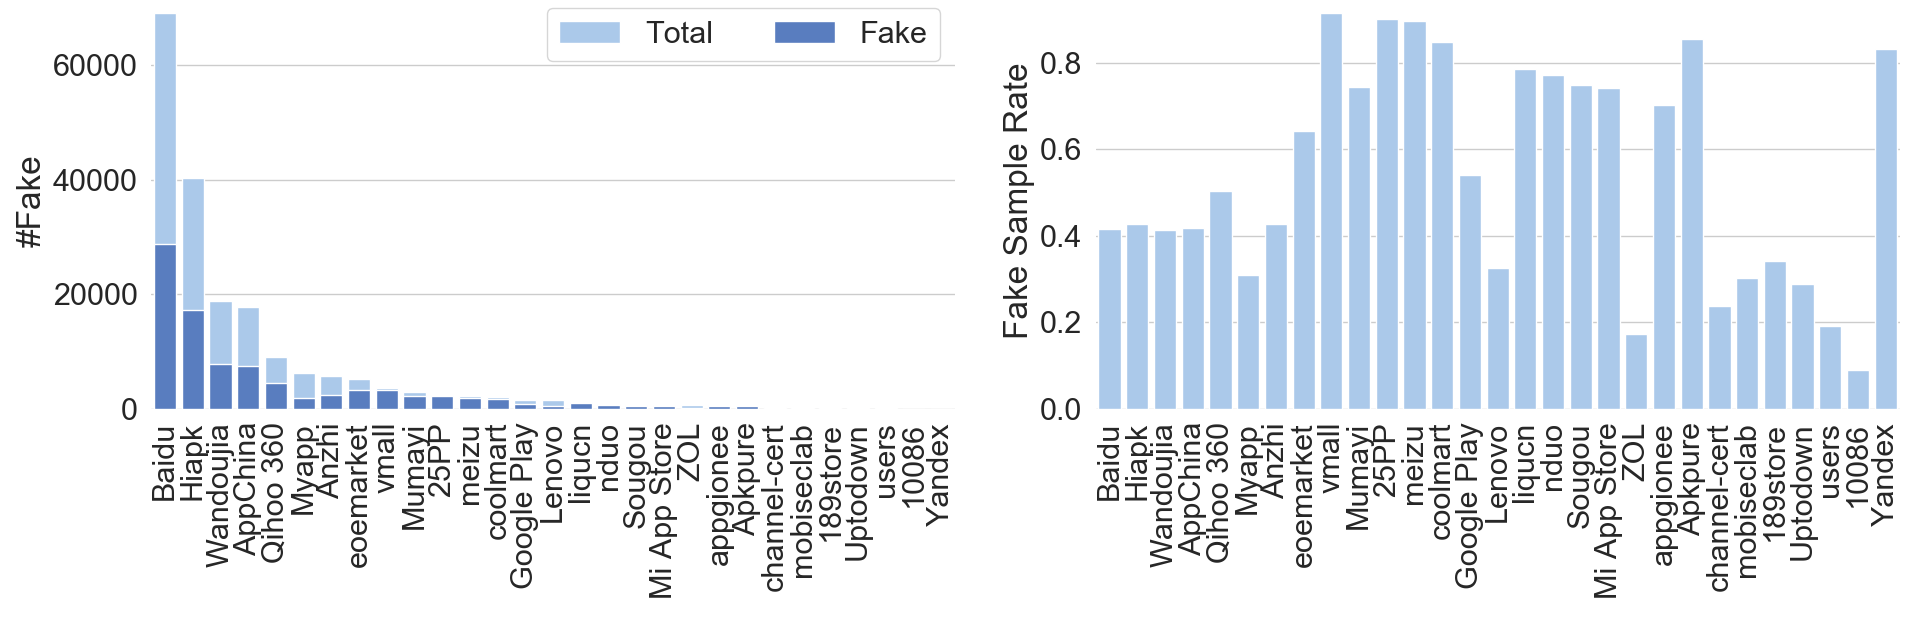
\includegraphics[width=\textwidth]{./Figures/edwin-Number_of_samples_collected_markets_3.png}
	\caption{Number of samples collected from different markets}
	\label{fig:Sample_source}
\end{figure*}

\noindent{\bf Answer to RQ 2.2.}
Intuitively, the more popular an app is, the more possible it would get shammed, for fake developers would mislead users to download their apps to gain profits.

Note that each app has different amount of samples (including official samples and fake samples), processing our measurement directly based on the number of fake samples is incorrect.
To counteract this bias, each fake count should be regularize into a \textit{fake sample rate}, the rate of fake samples in all collected samples of an app.

Next, we employ a metric called \textit{Pearson product-moment correlation coefficient (PPMCC)} to reveal relativeness between an app's fake sample number and its popularity, which uses the regularized fake sample rates and monthly activeness indicators (MAI) obtained from Analysys~\cite{yiguanqianfan}.
This value ranges from -1 to 1, the closer the PPMCC value is to 0, the weaker correlation between the two factors is indicated.
Surprisingly, according to our data, the value of PPMCC between this two factors is 0.246, revealing that the fake sample number and an app's popularity only hold their relativeness on a weak level, which does not match our expectation.

\noindent{\bf Answer to RQ 2.3.}
We assume the update frequency is related to the number of fake samples of an app, for updates can usually help keep a software from being attack.
The higher the update frequency is, the safer an app is supposed to be.

To estimate the average update frequency of our target apps, the time when an app's official sample was crawled and when its latest official samples were crawled is marked.
The difference between them is then divided by the number of that app's existing version to obtain an update frequency, with unit day/version.

The result PPMCC value of 0.084 shows that the connection between an app's update frequency and its fake sample rate barely exists.
We attribute this result to two reasons:
(1) The high update frequency (10 days/version on average for apps in our dataset) indicates app developers may not fix security issues in per update, weakening the function of update frequency as a security indicator.
(2) A large portion of fake samples in our dataset are not derived from repackaging. To this end, fake developers can produce fakes regardless of how well the official apps are protected.

\noindent{\bf Answer to RQ 2.4.}
Some categories are potentially more profitable than others.
A report from the app marketing company LIFTOFF~\cite{LIFTOFF_report} forecasts gaming to be the next most billable area.

Our 50 target apps are divided into 11 categories according to their functionalities, Table~\ref{table:data-statistics} shows these categories and their corresponding fake sample rate.
In the same category, the difference between apps on fake rate lies in an acceptable range.
Without doubt, entertainment related categories like \texttt{游戏} and \texttt{Social Network} attract more fake samples.
Another field, \texttt{Online shopping}, has also gained special love from fake developers because online shopping is rapidly developing in China.
Relatively, \texttt{商务办公} is not that attractive to fake developers, the average fake sample rate of this filed is only 4.05\%.
Apps in these four categories are marked in bold in the table.

The result matches the observation in our daily life, people always tend to use mobile devices for entertainment instead of business purpose.
It's pretty interesting to discover that the number of fake samples in a way reflects how people use their phone in their daily lives.

\vspace{1mm}
\noindent\fbox{
	\parbox{0.95\linewidth}{
		\textbf{Remark 2}: As revealed by statistics, the number of samples returned from an app store does not imply a fake rate.
		Additionally, the relationship between apps and market itself influences the number of fake samples from that market.
		To our surprise, an app's update frequency is not tightly correlated with its fake rate.
		We owe this to the fact that apps are updated too frequently and that repackaged samples are of minority in our dataset.
		We further observe that ``category'' as a factor has greater influence on the number of fake samples of an app than ``popularity'' and ``update frequency''.

	}
}

\begin{figure}
	\centering
	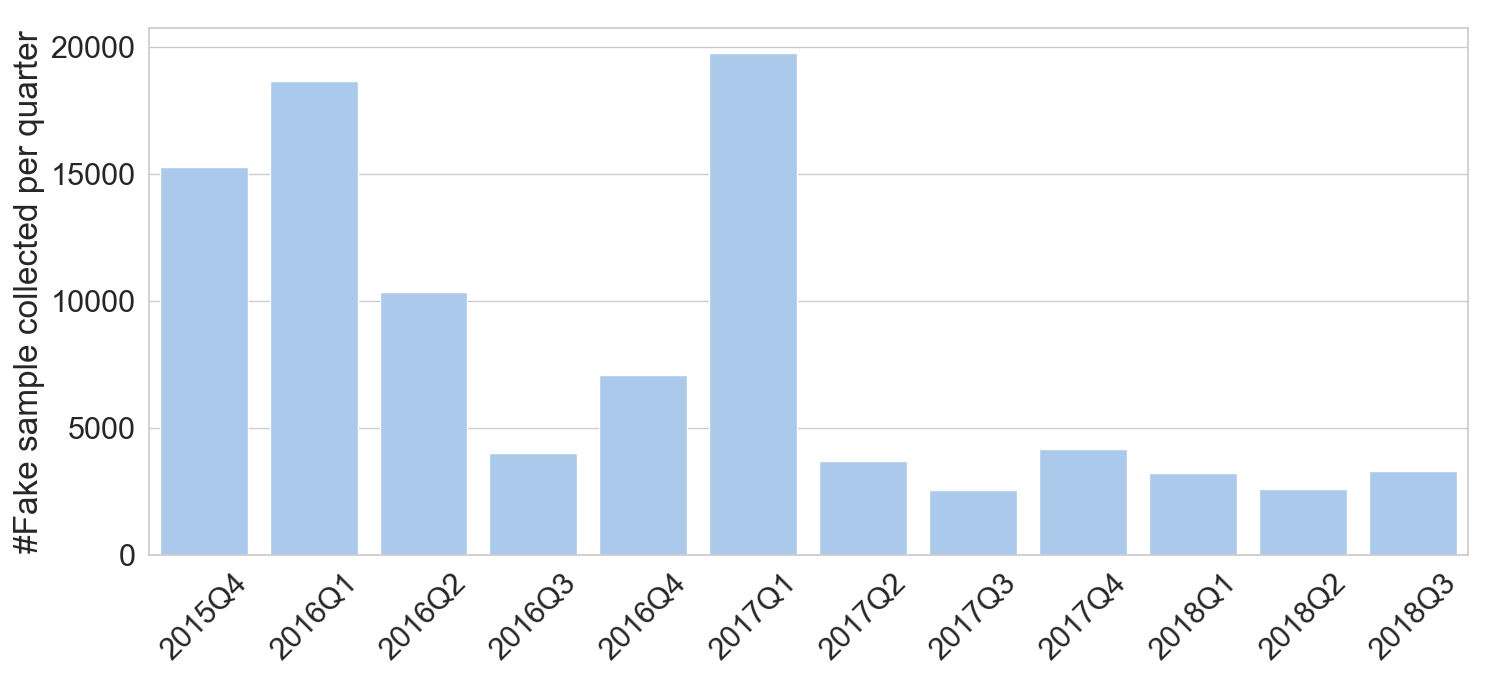
\includegraphics[width=\textwidth]{./Figures/edwin-Number_of_samples_collected_per_quarter_3.png}
	\caption{Numer of fake samples collected per quarter}
	\label{fig:Number_per_quarter}
\end{figure}

% \subsection{Developing Trend}
\section{Developing Trend}
In order to figure out fake apps' characteristics or behavior patterns over time, we propose the following research questions:

\noindent{\bf RQ 3.1} After a new version of an official app is published, how long do fake developers take to publish a new fake sample? In other words, how soon will these copycats appear?

\noindent{\bf RQ 3.2} How long can a fake app's certificate survive?

\noindent{\bf RQ 3.3} Is there a changing pattern of fake samples over time?


\noindent{\bf Answer to RQ 3.1.}
We compute this latency and show its distribution in Fig.~\ref{fig:Fake_latency_overall_distribution}.

Due to various reasons, it is hardly possible to retrieve the complete updating timeline for every single official app in our study, yet we approximately reproduce them with our data.
Firstly, we categorized all the official samples by their origins, and further categorized samples in each origin by version number.
After that, for each app and each version the samples are sorted by the date they were crawled, so by extracting the crawled date of the first sample in each version, we can obtain the earliest date a version is released.
Lastly, by combining and sorting the release dates of different versions according to different apps, we can reproduce the updating timelines of our target apps.

To find out the release latency of a fake app, all the dates on the timeline of the corresponding official app are compared in order to find out the smallest negative difference which we define as the release latency.
Fig.~\ref{fig:Fake_latency_overall_distribution} shows that most fake samples are published with the latency shorter than 20 days.
According to our statistics, 60\% of fake samples show up in 6 days after a new version of the official app is published.
This reveals a truth that fake developers are swift in action.


\noindent{\bf Answer to RQ 3.2.} Fig.~\ref{fig:Fake_certificate_survival_distribution} shows the distribution of the time a fake certificate can survive in markets.
In the left density distribution subplot, $x$-axes is the latency and $y$-axes shows the probability density of data at corresponding $x$ value.
%\edwin{mark.}
The total area under the curve is 1, and the area under two $y$ values $y1$ and $y2$ is the probability of their corresponding value $x1$ and $x2$ account for in data.
For example, in Fig.~\ref{fig:Fake_certificate_survival_distribution}, the area beneath curve between 0 to 200 on $x$-axes is close to 0.8, which means nearly 80\% of certificates only survive for no more than 200 days.

To judge how long a fake certificate can survive is similar to how we calculate the update frequency of an app, the first time and the last time a fake sample from the same certificate gets crawled are marked.
The time when a sample was crawled from a market might be different from the time when it is available in the market, but our crawler downloads new samples from different markets by days and we also use days as the unit in our measurement, so we can approximately regard this two values as the same one.

As shown in Fig.~\ref{fig:Fake_certificate_survival_distribution}, the distribution of fake certificate survival time shows that almost all the fake certificates live a short life, which means most fake certificates only show up in a short period of time.
This can be explained by a scheme that most markets have.
Once an app is found malicious or illegal, the market would stop that specific developer from uploading more samples by refusing to receive samples with the same certificate.
There are also a number of certificates which can survive for a long time.
According to the figure, some fake certificates even traverse the whole study interval.
We will conduct a case study on this phenomenon in Section ~\ref{sec:casestudy}.

\begin{figure}
	\centering
	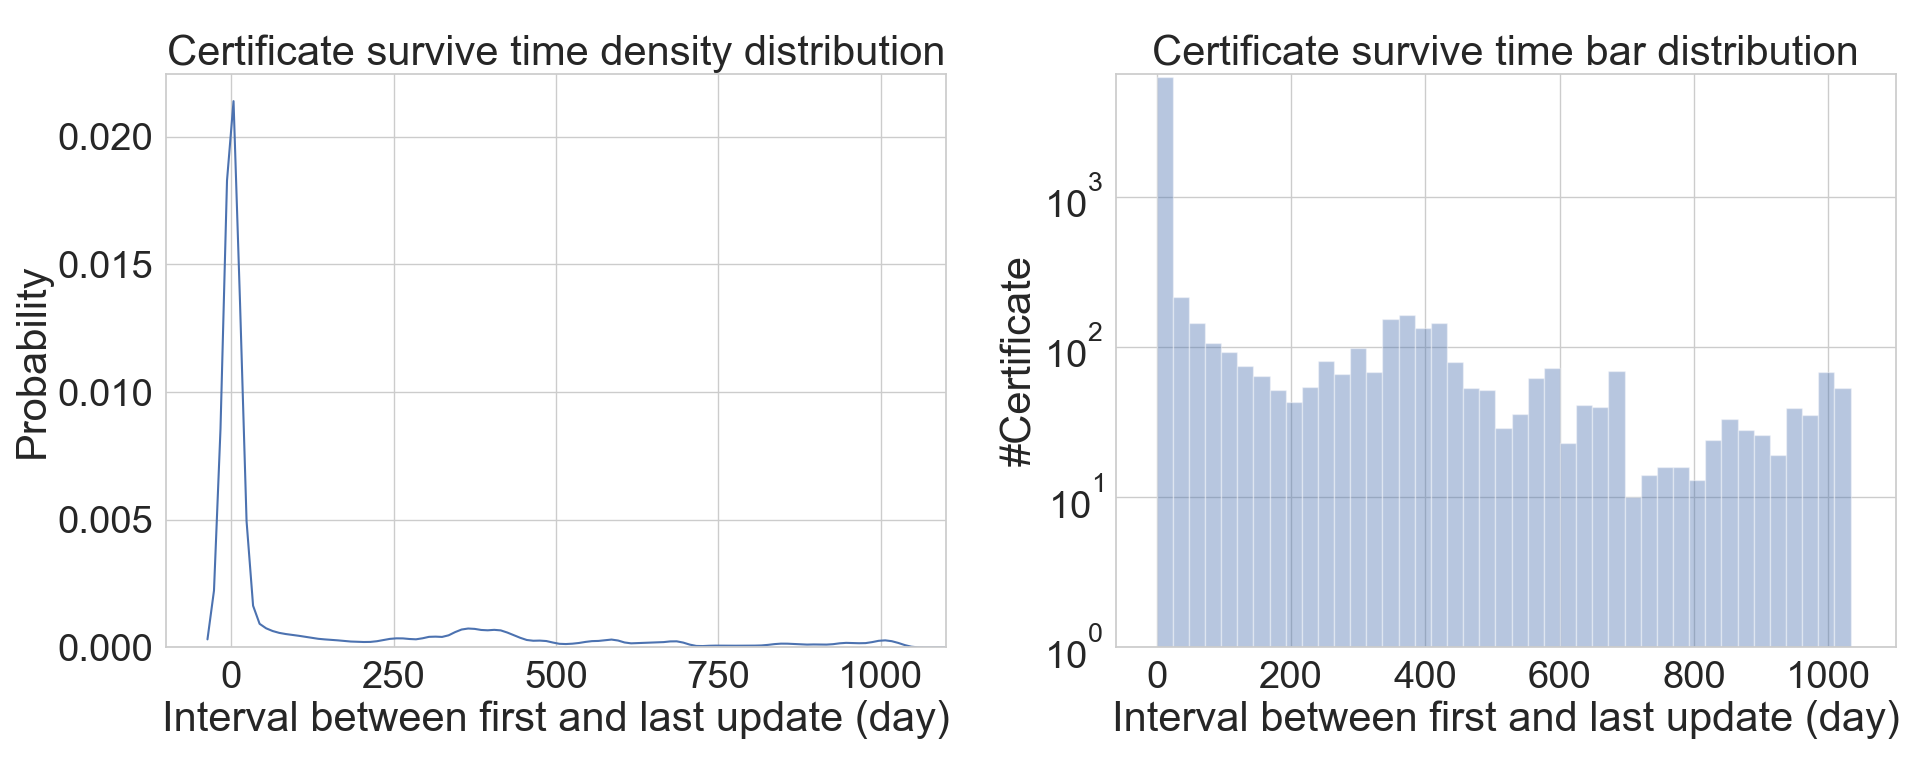
\includegraphics[width=\textwidth]{./Figures/edwin-Fake_certificate_survival_distribution2.png}
	\caption{Fake certificate survival time distribution}
	\label{fig:Fake_certificate_survival_distribution}
\end{figure}

\noindent{\bf Answer to RQ 3.3.} Fig.~\ref{fig:Number_per_quarter} shows the number of fake samples collected per quarter since the fourth quarter of 2015.
Although a large number of new fake samples get released in every quarter, the figure shows a tendency that the total number of fake apps on markets is gradually decreasing by years.
Note that our statistics only focus on fake samples, consequently this phenomenon does not indicate the underground industry is turning down.
Instead, we suppose this is possibly caused by the reform of fake apps.

On one hand, as stricter review schemes and stronger protection systems are applied on app stores, it's inevitable that fake apps in this study, become harder and harder to get on the shelf.
On the other hand, the new generation of malicious software, such as ransomware~\cite{ransomware} is impacting the underground industry.
Compare to fake apps, the new malicious apps are not only hard to defend (due to the innovative or even state-of-the-art techniques they utilize) but also extremely profitable.
Wannacry, a ransomware which was first spotted in the 2nd quarter of 2017, conquered tens of thousands of devices in a couple of weeks, which directly pulled up Bitcoin's price like a rocket~\cite{wannacry_bitcoin_news}.
Afterward, in the first quarter of 2018, a burst of cryptomining malware on phones emerged~\cite{comodo_report}.
This may be the reason why the number of fake samples suffers two suddenly drops in the second quarter of 2017 and the first quarter of 2018, respectively.


\begin{figure}
	\centering
	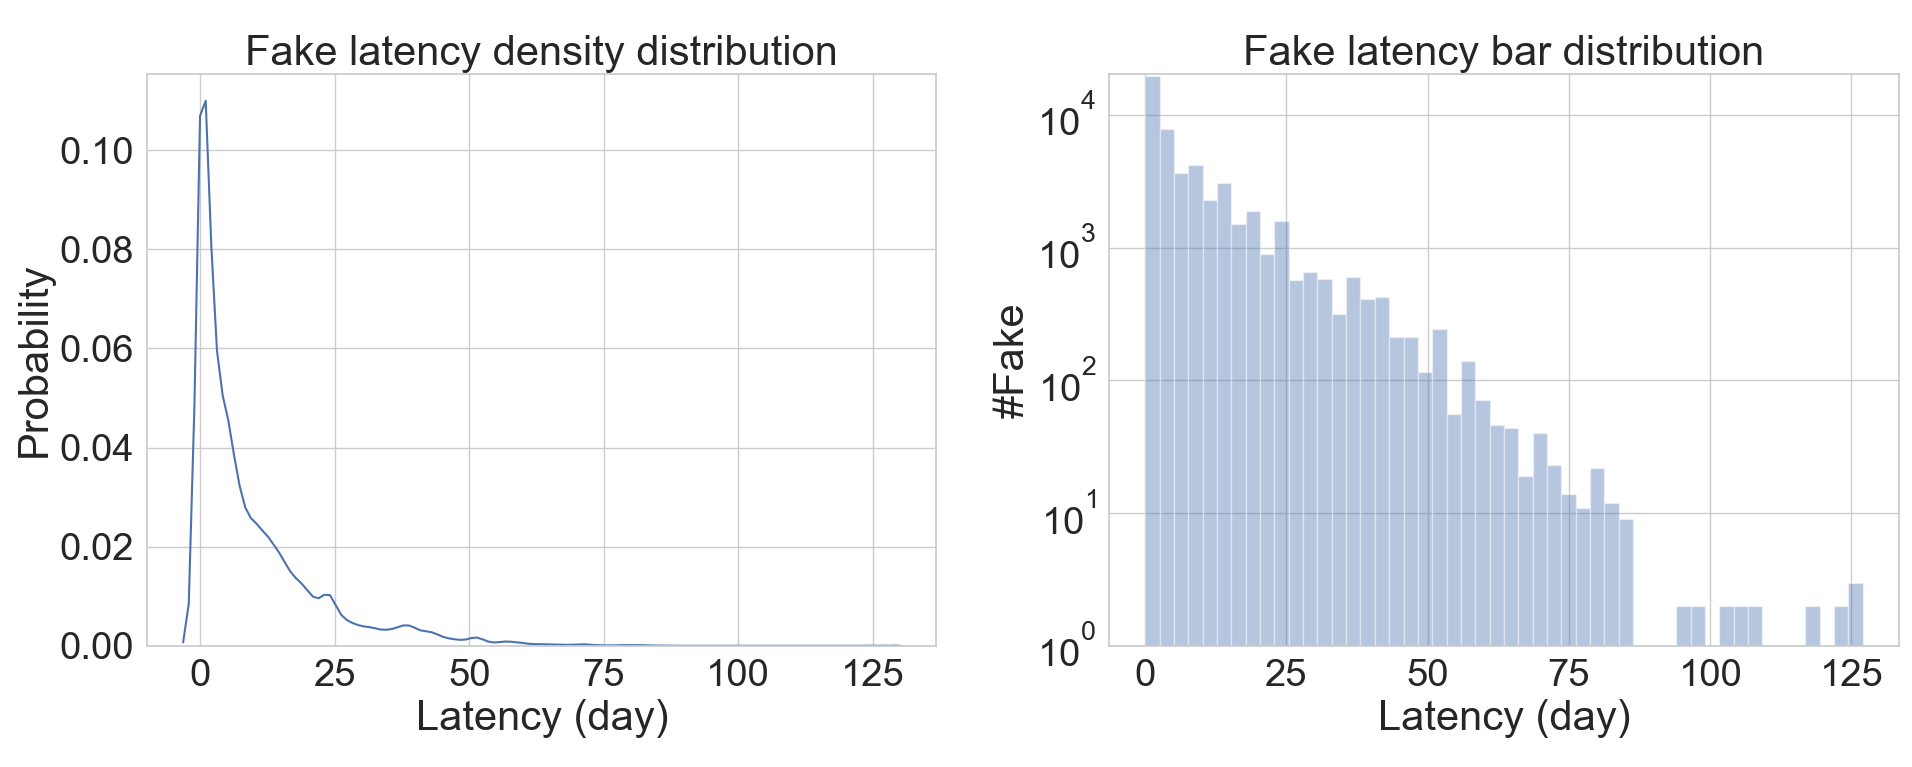
\includegraphics[width=\textwidth]{./Figures/edwin-Fake_latency_overall_distribution2.png}
	\caption{Fake latency overall distribution}
	\label{fig:Fake_latency_overall_distribution}
\end{figure}

\vspace{1mm}
\noindent\fbox{
	\parbox{0.95\linewidth}{
		\textbf{Remark 3}: Fake apps can be produced in a relatively short time, and the dropping number of fake samples by years suggests that they are mired in recession.
		Besides, only a few fake certificates survive for a long time, confirming that markets' protection schemes do work to some extent.
	}
}
